\documentclass{article}


\usepackage{inputenc}
\usepackage{url,hyperref}
\usepackage{paralist}
\usepackage{enumitem}
\usepackage{fancyhdr}
\usepackage{subcaption}
%for using image in document package%
\usepackage{graphicx}
\usepackage{colortbl}
\usepackage{amsmath}
\usepackage{algorithm2e}
\pagestyle{fancy}
%list of figures

\title{Artificial Intelligece and Machine Learning In Bangladesh Perspective}
\author{Avijit Chowdhury$^1$}

\date{
\small{
{ %
$^1$Chittagong University of Engineering and Technology,\\
Chattogram- 4369, Bangladesh\\%
    }}
    December 2024   }

% header and footer
\lhead{chapter 1}
\chead{Paper}
\rhead{1}
\renewcommand{\headrulewidth}{0 pt}

\lfoot{Copyright}
\cfoot{Avijit Chowdhury}
\rfoot{@}

\fancypagestyle{style}{\fancyhf{}\fancyhead[l]{\textit{Kazi Nazrul}}\fancyhead[c]{agnibina}\fancyhead[r]{2}
\fancyfoot[l]{\textit{Avijit Chowdhury}}\fancyfoot[c]{b}\fancyfoot[r]{2}
}
\setlength{\extrarowheight}{6 pt}
\begin{document}
\listoffigures

%list of table
\listoftables
\tableofcontents
\maketitle
\vspace{-1mm}
\begin{center}
    Greatest Scientific Innovation of the Century
\end{center}

\section{Introduction}
Lets begin with a formula \( e^{i\pi}+1 \). This \( \ln e^{x} \).
Computer vision is a field of artificial intelligence (AI) that uses machine learning and neural networks to teach computers and systems to derive meaningful information from digital images, videos and other visual inputs—and to make recommendations or take actions when they see defects or issues.

\subsection{Graphical Abstract}
\subsection{Keywords}
Artificial Intelligence, Machine Learning \cite{xiao2022novel}, Deep Learning, Neural Networks,
\section{Methodology}
This is the final project of my thesis project. So, I will be the first person
\small
will be the first person in this kind of complex project. hello\\
\large
lorem ipsum dolor sit amet, consectetur adip eget in eget \\
\huge
    elit. Duis sed libero non dolor bibendum tempor. \\
\tiny
\underline{nisi id fermentum ultricies, risus nunc varius tortor, ut convallis} \\
\large
\textbf{\textit{ lorem ipsum dollar smit}} \\
% এটি একটি ইংরেজি লেখা ছোট অধ্যায় যে বাঙ্গালী এ \textenglish{Google Translate} দ্বারা অনুবাদ করা হয়েছে. এটা খুব স্পষ্ট নয় যদি সঠিক অনুবাদ বা না কিন্তু ক্রিয়াটি ফন্ট দেখাতে যথেষ্ট হওয়া উচিত. \\
\$150 \\
\#1500 \\
\copyright \\
\textregistered \\
\begin{center}
Worlds best programmer
\end{center}
\begin{flushright}
    Avijit Chowdhury
\end{flushright}
\begin{flushleft}
    Avijit Chowdhury
\end{flushleft}

5 Qualities of a student
\begin{itemize}
\item Confidence
\item Hardworking
\item Punctuality
\end{itemize}

\begin{enumerate}
    \item Confidence
    \item Hardworking
    \item Punctuality
    \item Confidence
    \item Hardworking
\end{enumerate}

% Gold medalist in amth oplympiad
\begin{enumerate}
\item Bangladesh
    \begin{enumerate}
        \item Prakash
        \item Avijit
        \item Rony
    \end{enumerate}
\item India
\item Pakistan
\item Sri Lanka
\end{enumerate}

\begin{inparaenum}[a)]

\item Bangladesh
\item India
\item Pakistan

\end{inparaenum}

\section{Country}
\begin{enumerate}[label=\roman*]
\item Bangladesh
\item Bangladesh
\item India
\item Pakistan
\end{enumerate}

% hyperlink and url

\section{hyperlink and url}
\url{www.youtube.com} \\
\href{www.youtube.com}{Youtube}


% Customize the header and footer
\newpage
\section{second page}
\thispagestyle{style}


%Inserting image
%simple technique for inserting a new image
\begin{center}
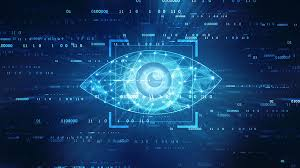
\includegraphics[scale=0.5]{vision.jpg}
\end{center}
%Inserting image with caption
%Adding h for the right position of the image in the document
\begin{figure}[h]
    \centering
    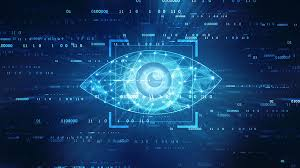
\includegraphics[scale=0.5]{vision.jpg}
    \caption{This is the vision of the project}
    \label{fig:vision}
\end{figure}
\section{About computer vision}
Computer vision is a field of artificial intelligence that trains computers to interpret and understand the visual world. Using digital images from cameras and videos and deep learning models, machines can accurately identify and classify objects and then react to what they "see." Computer vision technology is used in a variety of applications, including medical diagnosis, autonomous vehicles, and industrial quality control.
We can refer to the fig \ref{fig:vision} for the vision of the project.\\

%subfigure
\begin{figure}
    \centering
    \begin{subfigure}{0.4\textwidth}
        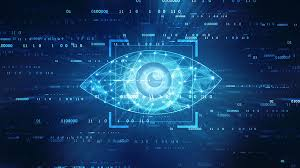
\includegraphics[scale = 0.5]{vision.jpg}
        \caption{Computer Vision}
        \label{fig:vision(a)}
    \end{subfigure}
    \begin{subfigure}{0.4\textwidth}
        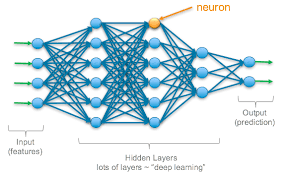
\includegraphics[scale = 0.5]{deeplearning.png}
        \caption{Deep Learning}
        \label{fig:dlearning(b)}
        
    \end{subfigure}
    \caption{Computer Vision and Deep Learning}
    
\end{figure}
\section{Deep Learning}
Deep learning is a subset of machine learning that uses artificial neural networks to model and solve complex problems.
\cite{zhou2021blockchain} It is called "deep" learning because it uses multiple layers of artificial neural networks to represent and learn data. Deep learning models can achieve state-of-the-art accuracy in tasks such as image recognition, speech recognition, and natural language processing.
We can refer to the fig. \ref{fig:dlearning(b)} for the deep learning of the project.\\
\section{Results}
%table
\begin{table}[h]
    \centering
    \begin{tabular}{|c|c|c|}
        \rowcolor{yellow}
        \hline
        \textbf{Model} & Accuracy & Precision\\
        \hline
        \hline
        \textbf{AlexNet} & 96 & 95\%\\
        \hline
        \textbf{ResNet50} & 97 & 98\%\\

    \hline
    \end{tabular}
    \caption{Performance of the deep learnig models}
\end{table}

%Mathmetical Expressions

\section{Mathematical Expressions}
Mathematical Expressions for the deep learning \ref{eq:e} and \ref{eq:ln} and \ref{eq:frac} and \ref{eq:lim} are given below.\\
\begin{equation}
    e^{i\pi}+1 = 0
    \label{eq:e}
\end{equation}

\begin{equation}
    \ln e^{x} = x
    \label{eq:ln}
\end{equation}

\begin{equation}
    \frac{1}{2} \times 5 = 2.5
    \label{eq:frac}
\end{equation}

\begin{equation}
    \lim_{a \rightarrow 7} f(a)
    \label{eq:lim}
\end{equation}

\begin{equation}
    \int_{0}^{\infty} \frac{\sin {x}}{\tan {{x}^{2}}} dx_2
    \label{eq:int}
\end{equation}

\begin{align*}
    a & = b + c \\
   c & = d + e \\
   e & = f + g \\
\end{align*}

% or you can use split
\begin{equation}
    \begin{split}
        a & = b + c \\
        c & = d + e \\
        e & = f + g \\
        \alpha &= 30  \\
        \beta &= 45 \\
        \gamma &= 60  \\
        \delta &= 90  \\
    \end{split}
    \label{eq:eqs2}
\end{equation}

%matrix
\begin{equation}
    \begin{bmatrix}
        1 & 2 & 3 \\
        4 & 5 & 6 \\
        7 & 8 & 9 \\
    \end{bmatrix}
\end{equation}



\section{Discussion}
\section{Conclusion}
\section{Acknowledgement}


\bibliographystyle{ieeetr}
\bibliography{ref.bib}
% \section{References}
% \begin{thebibliography}{9}
% \bibitem{1} Avijit Chowdhury, 2024, "Artificial Intelligence and Machine Learning", Springer
% \bibitem{2} Avijit Chowdhury, 2024, "Artificial Intelligence and Machine Learning", Springer
% \bibitem{3} Avijit Chowdhury, 2024, "Artificial Intelligence and Machine Learning", Springer
% \bibitem{4} Avijit Chowdhury, 2024, "Artificial Intelligence and Machine Learning", Springer
% \bibitem{5} Avijit Chowdhury, 2024, "Artificial Intelligence and Machine Learning", Springer
% \bibitem{6} Avijit Chowdhury, 2024, "Artificial Intelligence and Machine Learning", Springer
% \end{thebibliography}




\end{document}
\end{document}